\documentclass{beamer}
\usepackage{xcolor}
\usepackage{polyglossia}
\setmainlanguage{spanish}
\setmainfont
[Ligatures=TeX, % recommended
UprightFont={*},
ItalicFont={* Italic},
BoldFont={* Bold},
BoldItalicFont={* Bold Italic}]
{Fira Sans}
\setsansfont
[Ligatures=TeX, % recommended
UprightFont={*},
ItalicFont={* Italic},
BoldFont={* Bold},
BoldItalicFont={* Bold Italic}]
{Fira Sans}
\setmonofont{Fira Mono}
\newfontfamily\FiraTitle
[Ligatures=TeX, % recommended
UprightFont={* Heavy},
BoldFont={* Ultra}]
{Fira Sans}
\definecolor{green}{HTML}{4BCDAD}
\definecolor{purple}{HTML}{2F018D}

\title{\resizebox{\columnwidth}{!}{{\FiraTitle \textbf{\texorpdfstring{\textcolor{black}{Git}}{Git} \texorpdfstring{\color{green}{+}}{+} \texorpdfstring{\textcolor{purple}{Github}}{Github}}}}}
\subtitle{\resizebox{0.5\columnwidth}{!}{\FiraTitle \texorpdfstring{\textcolor{black}{De 0 a 100 en una clase}}{De 0 a 100 en una clase}}}
\institute{Universidad de Guanajuato}
\author{{\FiraTitle \texorpdfstring{\textcolor{black}{Mario Alejandro Gil Lázaro}}{Mario Alejandro Gil Lázaro}}}
\date{}

\setbeamercolor{frametitle}{fg=green}

\begin{document}

\frame{\titlepage}

\begin{frame}
  \frametitle{Tabla de contenidos}
  \tableofcontents
\end{frame}

\begin{frame}
  \frametitle{{\FiraTitle \textbf{Introducción: Sistemas de Control de Versiones}}}
  \begin{columns}
    \column{0.5\textwidth}
    {\FiraTitle Beneficios}
    \begin{itemize}
      \item Historial de cambios para todos los archivos
      \item Branching y merging
      \item Rastreabilidad
      \end{itemize}
    \column{0.5\textwidth}
    \begin{figure}
      \centering
      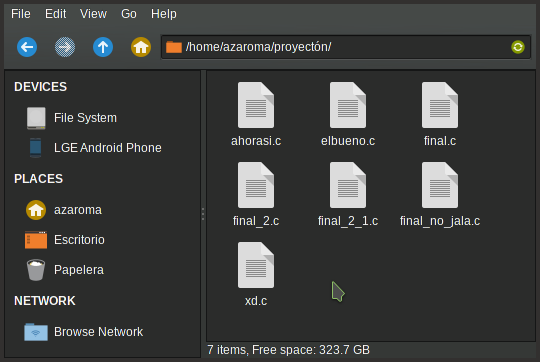
\includegraphics[width=\textwidth]{version}
      \caption{Control de versiones antiguo}
    \end{figure}
  \end{columns}
\end{frame}

\begin{frame}
\frametitle{Git}
\end{frame}

\begin{frame}
\frametitle{Repositorio}
\end{frame}

\begin{frame}
\frametitle{Add}
\end{frame}

\begin{frame}
\frametitle{.gitignore}
\end{frame}

\begin{frame}
\frametitle{Commit}
\end{frame}

\begin{frame}
\frametitle{Branch}
\end{frame}

\begin{frame}
\frametitle{Merge}
\end{frame}

\begin{frame}
\frametitle{Github}
\end{frame}

\begin{frame}
\frametitle{Remote}
\end{frame}

\begin{frame}
\frametitle{Clone}
\end{frame}

\begin{frame}
\frametitle{Pull}
\end{frame}

\begin{frame}
\frametitle{Push}
\end{frame}

\begin{frame}
\frametitle{Flujo de trabajo}
\end{frame}

\begin{frame}
\frametitle{Observaciones finales}
\end{frame}

\begin{frame}
  \frametitle{Referencias}
\end{frame}

\end{document}
